%\documentclass[letterpaper,10pt,titlepage]{IEEEtran}
%\documentclass[10pt, oneside,onecolumn,draftclsnofoot]{IEEEtran}
\documentclass[10pt,journal,compsoc,onecolumn, draftclsnofoot]{IEEEtran}

% \usepackage{graphicx}
% \usepackage{amssymb}
% \usepackage{amsmath}
% \usepackage{amsthm}
% \usepackage{caption}
%
% \usepackage{alltt}
% \usepackage{float}
% \usepackage{color}
% \usepackage{url}
%
% \usepackage{balance}
% \usepackage[TABBOTCAP, tight]{subfigure}
% \usepackage{enumitem}
% \usepackage{pstricks, pst-node}
%
% \usepackage{geometry}
% \usepackage{pst-gantt}
% \usepackage{tabu}
%
% \geometry{textheight=8.5in, textwidth=6in}
%
% %random comment
%
% \newcommand{\cred}[1]{{\color{red}#1}}
% \newcommand{\cblue}[1]{{\color{blue}#1}}
%
% \graphicspath{ {diagrams/} }
%
% \usepackage{hyperref}
% \usepackage{geometry}
% \usepackage{array}
% \usepackage{titling}

\def\name{Jake Jeffreys, McKenna Jones, Spike Madden, Sean Marty}
\title{
EmbarkVR: Outdoor Virtual Reality Experience \\
CS Senior Capstone \\
Design Document\\
\vspace{1mm}
}
\author{Jake Jeffreys, McKenna Jones, Spike Madden, Sean Marty}
\date{December 2nd, 2016}

%pull in the necessary preamble matter for pygments output

%% The following metadata will show up in the PDF properties
\hypersetup{
  colorlinks = true,
  linkcolor = black,
  urlcolor = black,
  pdfauthor = {\name},
  pdfkeywords = {cs461 ``senior capstone''},
  pdftitle = {CS 461 Design Document},
  pdfsubject = {CS 461 Design Document},
  pdfpagemode = UseNone
}

\begin{document}
\begin{bibunit}
\begin{titlepage}
\maketitle
\vspace{1mm}
\begin{abstract}
This document describes the design components of Intel and Columbia's virtual reality project. It is structured as follows. A brief overview section will outline the purpose, intended audience, definitions and project context. This is followed by the body of the document which further details the design of the project. The design description defines the stakeholders, views and viewpoints defined in the IEEE 1016 format. The project was broken up into four components: static environment, animation, Columbia gear integration and fishing rod mechanics. Each of these sections are discussed in depth in terms of design description.
\end{abstract}
\vspace{1cm}

\noindent\begin{tabular}{ll}
\makebox[2.5in]{\hrulefill} & \makebox[2.5in]{\hrulefill}\\
Intel Sponsor & Date\\[5ex]% adds space between the two sets of signatures
\makebox[2.5in]{\hrulefill} & \makebox[2.5in]{\hrulefill}\\
Columbia Sponsor & Date\\[5ex]% adds space between the two sets of signatures
\makebox[2.5in]{\hrulefill} & \makebox[2.5in]{\hrulefill}\\[2ex]
\makebox[2.5in]{\hrulefill} & \makebox[2.5in]{\hrulefill}\\[2ex]
\makebox[2.5in]{\hrulefill} & \makebox[2.5in]{\hrulefill}\\[2ex]
\makebox[2.5in]{\hrulefill} & \makebox[2.5in]{\hrulefill}\\
Student Team Members & Date\\
\end{tabular}

\end{titlepage}
\tableofcontents
\clearpage

\section{Overview}
\subsection{Scope}
We want to create an outdoor virtual reality experience for customers at a Columbia retail store. The application will consist mainly of visual, audio, and tactile experiences to create an outdoor world in which the user can navigate. The main activities available will involve fly fishing in one of the rivers and interacting with virtual Columbia products while in the experience to gain specific product information.

\subsection{Purpose}
The main goal of the project is to make customers feel more inclined to purchase Columbia gear through the use of an immersive, outdoor virtual reality experience. This document exists both for development of the project and to provide a detailed description of the design plans.

\subsection{Intended Audience}
The intended audience of this design document are the student developers involved (EmbarkVR), project sponsors, and Capstone teachers. The development team will be using this report as a guide and will provide structure for the development process. The sponsors can use this document to understand the vision of the developers and it will give a platform to discuss design ideas. The teachers can benefit from this document by learning about the project as a whole.

\section{Definitions}
\begin{itemize}
  \item Virtual Reality (VR):  Artificial environment that is created with software
  \item HTC Vive: A virtual reality system produced by HTC
  \item Base Stations: These allow the Vive to track the movement and location of the controllers and headset.
  \item Wands: Controllers that are used with the Vive headset.
  \item Unity Game Engine: The Unity Game Engine, developed by Unity Technologies is used in this project to develop the virtual reality simulation.
  \item GameObject: The base class for all entities in Unity scenes.
  \item GitHub: Web-based Git repository hosting service
  \item Git: version control system used for software development
\end{itemize}

\section{Project Context}
\subsection{Hardware}
\begin{itemize}
  \item Computer with the following specifications:
  \begin{itemize}
    \item Processor: Intel Core i5-4590 or AMD FX 8350, or better
    \item Graphics: NVIDIA GeForce GTX 1060 or AMD Radeon RX480, or better
    \item Memory: 4GB RAM or better
    \item Operating system: Windows 7 SP1 or better
  \end{itemize}
  \item HTC Vive Headset: Used to track head movements and display application to users.
  \item HTC Wands (x2): Used to track the users hand movements and to give the user the ability to interact with virtual objects within the application.
  \item HTC Base Stations (x2): Used to track location of headset and wands. This information is then sent back to the computer in real time.
\end{itemize}
\subsection{Software}
\begin{itemize}
  \item Unity Gaming Engine: Used to develop the application.
  \item Unity Asset Store: Used to find objects which can be imported into the application.
  \item GitHub: Used by developers to collaborate and share files.
\end{itemize}


\section{Design Description}
The following will discuss the stakeholders, views, viewpoints, and rationale behind the design of the project.
\subsection{Design stakeholders}
\subsubsection{Intel}
In this project, Intel is working with Columbia Sportswear to help them meet their needs.
Intel has graciously provided all necessary hardware to our team to allow us to create a successful application.

\subsubsection{Columbia Sportswear}
One aspect of Columbia Sportswear is their fishing apparel.
Specifically, the Performance Fishing Gear (PFG) line of apparel.
Columbia hopes to use the application we are developing in a retail store to showcase the PFG line in a new medium.
The goal is to inspire customers to try new outdoor activities with Columbia gear.

\subsection{Design views}
\subsubsection{Users}
Users of the product expect this virtual reality experience to be as realistic and immersive as possible. We will be making the assumption that users will be experiencing this application with out any previous virtual reality or fly fishing experience. We are making this assumption to account for everyone who may be interested in participating. From their perspective, they will care most about their ability to quickly understand how to move around and interact with objects. This means that we need to create intuitive tools and controls. Users can also expect to find visual queues and instructions within the experience.

There are two main perspectives that users will have when using this product.
Firstly, users will be hoping to gain an outdoor experience that they might not otherwise have the opportunity to try. Therefore, realism is key in this view.
Secondly, users will expect interaction with Columbia gear in a meaningful way.
The user should leave the experience with a feeling of how the Columbia gear would perform in a certain environment.

\subsubsection{Intel Sponsor (Mike Premi)}
The Intel sponsor of the project, Mike Premi, is concerned more with the technical side of the project.
Things like which technologies are used, the technical performance, and overall technical design considerations are all important under this view.
This view will guide the design process on a technical level.

One of the main goals of the project is to make the experience as immersive and realistic as possible. To achieve this we will first need to use a high performance computer. Second, we will need to constantly be aware of performance restrictions during the development process, mainly while improving realism. The realism techniques we discuss later in this document will all take a toll on performance speeds and application responsiveness.

\subsubsection{Columbia Sponsor (Tim Devlin)}
The Columbia Sportswear sponsor of the project, Tim Devlin, is concerned primarily with the how the user will interact with Columbia products in the Virtual Reality experience.
This includes, how products are displayed, what information related to the products is shown, and the user interaction with said products.
Ultimately, the goal of the product under this view is to create more sales for Columbia Sportswear.
Therefore, that is what is most important under this view.
This view will guide the design process at a higher level compared to the view of the Intel Sponsor.

\subsection{Design viewpoints}
\subsubsection{Context viewpoint}
This context is related to user interaction within the application in the
environment. It provides a "black box" view of the project which can be useful
from the perspective of users. From the perspective of the user,
everything should be intuitive and they should rarely notice any issues with
frame rate.\\

\hangindent=0.5cm \textbf{Design Concern}: The main concern will come from
users of the VR application. The ability to interact seamlessly with the application is
essential. Users do not want to experience performance lag or errors in functionality.
They also should not need to ever leave the application to ask questions about how to
perform tasks or interact with objects. It must be an intuitive application
that is easy to understand in less than 30 seconds given a minor introduction
beforehand. \\

\hangindent=0.5cm \textbf{Analytical Methods}: Once we have a fully functioning
prototype we will put our application through user testing. During the testing
phase the application will be evaluated on the basis of immersion, enjoyment,
and possibly influence over customer purchase decisions. After users test the
application we will ask for feedback related to their experience in the form of
oral questions or an anonymous written survey depending on what the user
prefers. \\

\hangindent=0.5cm \textbf{Rationale}: We included this viewpoint due to the importance of user immersion. The user experience in virtual reality applications is very sensitive and there are many factors that can influence it. According to a study done by Intel and Thug\cite{michalak_lind_round1}, immersion needs graphical fidelity, not realism. They found that what was important was crisp and clean graphics at all times. They also found that a smooth experience, one without glitches and lost frames, was the most important aspect of immersion. They even went a step further to argue that photo-realism is often times worse because it makes inaccuracies more obvious.

\begin{figure}[h]
\centering
\caption{Context Viewpoint Diagram}
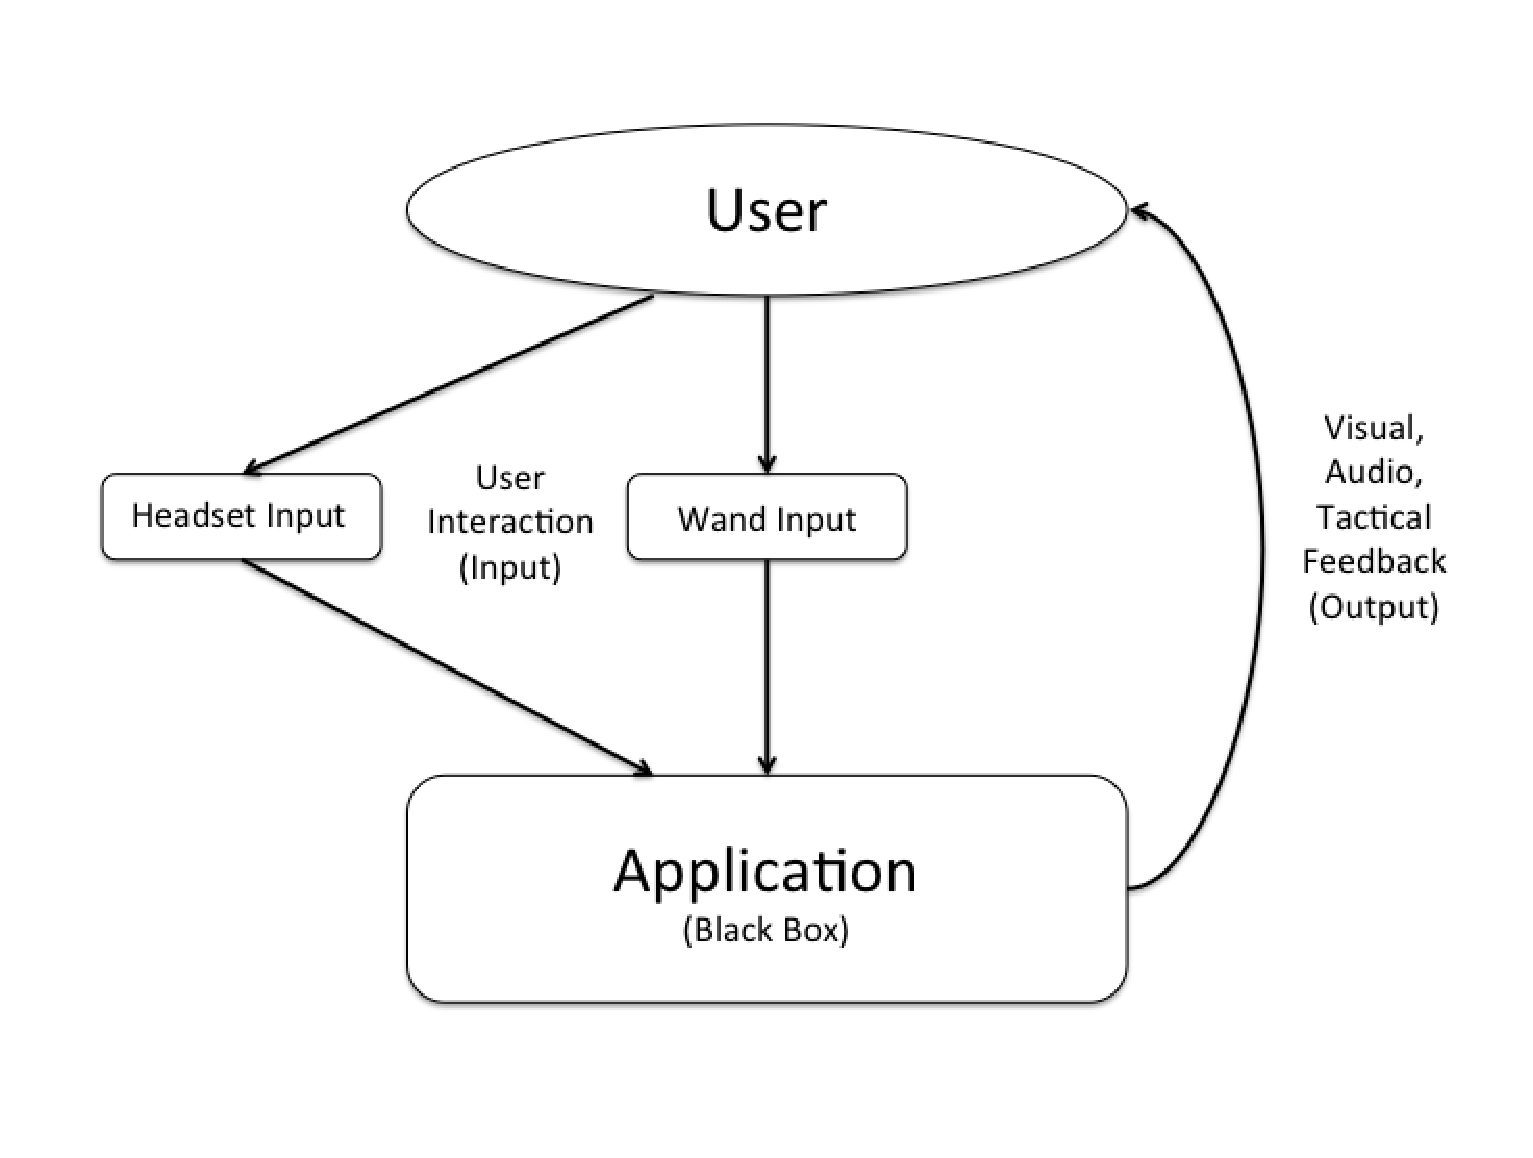
\includegraphics[width=0.8\textwidth]{projectContext.eps}
\end{figure}

\subsubsection{Composition viewpoint}
Project composition is the organization of, and relationships between, each of
the sections of our project. Each portion of the project will be explored in
more detail in the Approach section below, but our virtual reality experience
will be the sum of visual and audio assets, scripts, game objects, and HTC Vive
hardware. All of this will be integrated to create a single, powerful retail
experience.\\

\hangindent=0.5cm \textbf{Design Concern}: The composition of the project affects ease of implementation, performance, and how well an outside developer can come in
and familiarize themselves with the project. The Intel Sponsor Mike Premi will
find this viewpoint important because of his role in guiding our technical
development. Also, the Columbia Sponsor, Tim Devlin will find this viewpoint
valuable because once the product is applied in a retail setting, a well-composed project
will ease the transition and replication.\\

\hangindent=0.5cm \textbf{Analytical Methods}: It will be hard to objectively analyze the success of this viewpoint, but the effects of a well or poorly composed project will
undoubtedly be seen throughout development and implementation. A good test of
quality composition will occur whenever parts of the project need to be
passed from one team member to another, or from the team to an outside
developer. Project composition will be one of the factors in how well these
transfers go.\\

\hangindent=0.5cm \textbf{Rationale}: We included the composition viewpoint because there are going to be a massive number of assets, scripts, and objects involved in the
production of this virtual reality experience. It is vital to have our design
keep an eye on composition so that nothing gets lost in the complexity of the
undertaking. Also, as our team learns and improves our product, there will be
periods of redesigning and modification that need to stay within the planned
composition in order to not break other portions of the project.

\begin{figure}[h]
\centering
\captionsetup{justification=centering}
\caption{Composition Viewpoint Diagram}
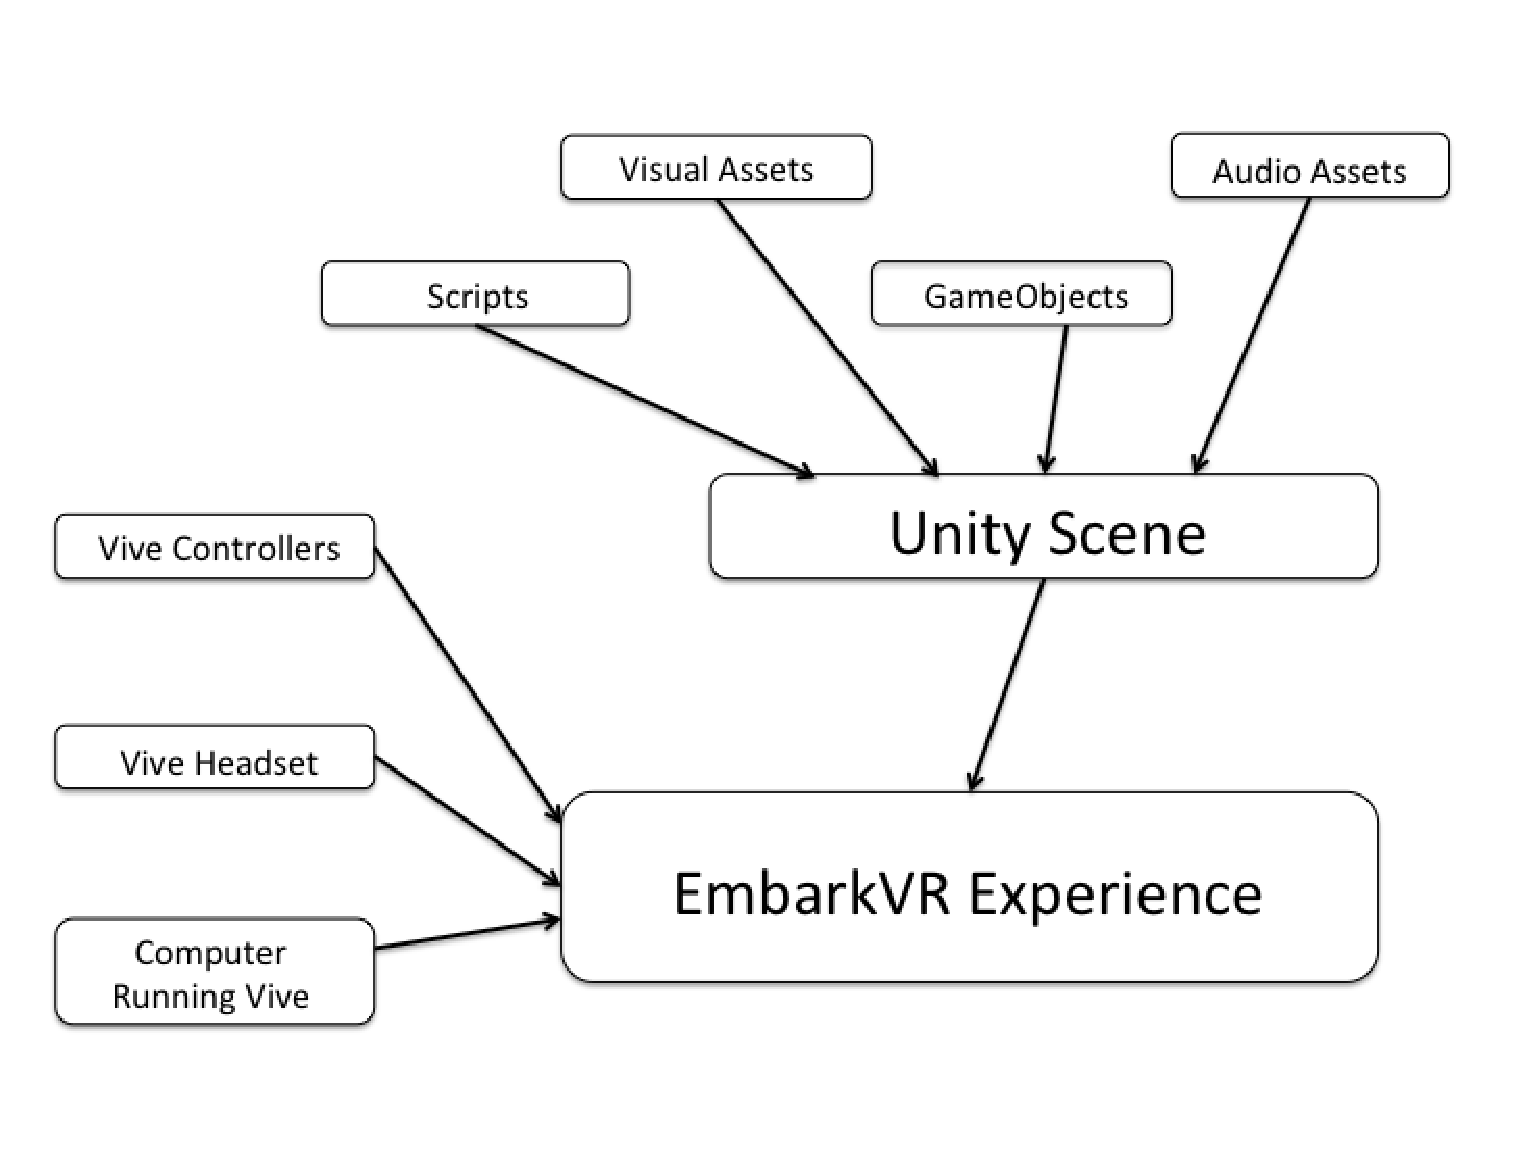
\includegraphics[width=0.8\textwidth]{projectComposition.eps}
\end{figure}


\subsubsection{Dependency viewpoint}
The Dependency viewpoint specifies the relationships of interconnection and access among entities. These relationships include shared information, order of execution, or parameterization of interfaces. Establishing these relationships will be key in organizing the project's workflow.\\

\hangindent=0.5cm \textbf{Design Concern}: Users will appreciate fluid and thoughtful interaction between assets within the virtual reality system. Both Intel sponsor Mike Premi and Columbia sponsor Tim Devlin will want clear dependencies to be outlined before any development begins to prevent any redundancies. This will save both time and resources during development and will result in a clear, aligned final product.\\

\hangindent=0.5cm \textbf{Analytical Methods}: We will be able to find any dependency issues during development as certain components will not be functional without others. Development will halt any time a dependency issue arises that needs to be resolved. Ultimately, user testing with the final product will determine if the dependencies we outlined were implemented correctly.\\

\hangindent=0.5cm \textbf{Rationale}: We included the dependency viewpoint because of the importance of planning ahead in a large software development project such as this. Design of the four major components, static assets, animation of the environment, rod mechanics, and Columbia gear integration are going to heavily rely on each other and need to be accounted for. The static environment will most likely be developed first, followed by the animation. Rod mechanics and Columbia gear integration will depend on both the created environment and available assets and animation. Successfully consolidating these elements will result in a polished final product.\\

\subsubsection{Interface viewpoint}
Within this project there are a number of interfaces, external and internal, that both the users and developers will be working with.
The purpose of this viewpoint is to make it extremely clear how all of the interfaces work together to create a final product. \\

\hangindent=0.5cm \textbf{Design Concern}: This viewpoint is primarily addressed at the technical side of the project.
Therefore, the view with most interest in this viewpoint is the Intel Sponsor, Mike Premi.
The main external interfaces are the HTC Vive system, which includes the headset, controllers, and base stations, the computer where the software is running, and any external monitors that are being used.
As for internal interfaces, the project will involve the Unity Game Engine, SteamVR, and Visual Studio for C\# development.
In the short term, developers are most concerned with the interfaces, but long term, users will also see the impacts of the interface viewpoint.
The orchestration of all interfaces is essential to creating a complete final project. \\

\hangindent=0.5cm \textbf{Analytical Methods}: The creation of a product that works without any major issues depends on this viewpoint.
All interfaces must play nicely with each of their dependencies for this to happen.
During the design and development of the project, this viewpoint will guide the developers by providing an understanding of which interfaces of the project are important for each component.
An indicator of good interface design will be if there are no interfaces which inhibit the functionality of other interfaces.\\

\hangindent=0.5cm \textbf{Rationale}: This viewpoint was included because of the range of technologies that are used within the project.
The way interfaces interact will affect users indirectly, and those with technical interests in the project directly.

\subsection{Design Rationale}
We chose to use the Unity gaming Engine to build our project. Here are some of the reasons for our decision:
\begin{itemize}
  \item A large community base
  \item Compatible with Mac, Windows and Linux operating systems
  \item A relatively small learning curve, good for projects with a small time frame
  \item Built-in support for various VR related functions
  \item Includes a large, free asset store
  \item Uses C\# as its scripting language, a language that our team has experience with
\end{itemize}

\section{Approach}
\subsection{Static Environment}
The basis of our virtual reality experience is the underlying static
environment. Before we can start any animation, lighting, audio or physics
work we need to build up a static terrain and collection of 3D objects.
Most components of the environment will not just be static, but they will all
start out that way when they are brought into our project. The basic project
building block in Unity is a scene, which can be thought of as a level in a
video game. \cite{microsoft_mag} For our experience, the initial design will
only have one scene because there isn't built-in user movement. This means that
every object, texture, and script in our environment will exist within the
scope of this single scene.

\subsubsection{Concerns}
This project component is most important from a dependency viewpoint.
Before other aspects of the project can be completed, there needs to exist a static environment.

\subsubsection{Approach}
The main sections of the approach for this component are the static terrain, the realism of said terrain, static objects incorporated into the terrain, and finally assets used for the static environment.\\

\hangindent=0.5cm \textbf{Static Terrain}: When building our static environment, we
will start with the basic Unity terrain engine. A terrain object in Unity starts out
as a flat plane, and then can be painted on with various
effects.\cite{unity_man_terrain} These effects include heightmap effects and
textures. In our environment, this will mean bringing out a riverbed, shore, and
surrounding features such as hills with the heightmapping tool. Next up is adding
base textures. Just adding a 2D texture for, say, grass will not provide nearly the
level of authenticity we want the user to feel, so we will not use these textures
for more than a base or background to 3D objects.\\

\hangindent=0.5cm \textbf{Static Realism}: In the next section we will cover
animation and realism through effects, but a certain amount of realism can be
achieved just by careful choice of our static environment arrangement. We will do
research on real world locations for fly fishing and draw from that as much as
possible. For example, it is tempting to place trees in our environment in a
semi-random, evenly spaced pattern or something similar. However, it will increase
our authenticity if we base our placement choices on what actually occurs in nature.
This is one example, but it demonstrates a larger theme, which is that because we
are only producing a single scene and we want it to be as real as possible,
attention to every reasonable detail is key.\\

\hangindent=0.5cm \textbf{Static GameObjects}: Now that we have a terrain set up,
the next step is to add static objects to the environment. At the most basic, Unity
uses the GameObject type for all objects, and those objects have subobjects and
components associated with them. \cite{ray} Without going into much detail about the
actual workings of objects in Unity, there are two main aspects of game objects that
we will use in our development to make our lives easier. Both of these features help
solve problems that come with an environment that will contain lots of similar
objects such as trees, stones, or grass. First, we will use prefabs to easily
edit similar settings on a whole group of objects and make replication much
easier. \cite{ray} Second, objects can be grouped into layers, which will
provide us with the ability to toggle whole sections of our environment by
theme while in development. \cite{layers_video} It will be helpful to be able
to one-click toggle layers such as trees or small animals to clear up and
expose underlying features.\\

\hangindent=0.5cm \textbf{Static Assets}: It is perfectly good to be able to populate our environment with static objects but now we will need to actually create those visual 3D objects. In Unity, all project assets go into one central folder, which is brought into the editor for use. \cite{unity_importing_assets} There are all kinds of asset sources that we will explore, including specific Columbia asset files that will be provided by Columbia through Tim Devlin. Importing a quality set of assets will be the last step in creating a vibrant, realistic static environment to work with in our experience.\\

\subsection{Improve Realism and Animate Environment}
One of the main goals of our project is to make it as realistic as possible
without compromising performance. Realism can come from a number of different
techniques.
\subsubsection{Concerns}
From a dependency viewpoint it is important to have a static environment already created. However, in order to build a static environment we need to be aware of how dynamic textures work to effectly combine these two concepts.

\subsubsection{Aspects}
The three techniques we will be focusing on when it comes to improving realism are animation, audio, and lighting. \\

\hangindent=0.5cm \textbf{Animation}: First we will be focusing on is environment animation. A majority of our application will take place in a river so we will need to make this river as animated as possible. This will involve an animation of the water moving passed the users and can be done using an open-source animated water shading. A similar technique can be used to create movement of clouds in the sky.\\

\hangindent=0.5cm \textbf{Audio}: The next step to improving realism is adding audio. Audio is crucial when it comes to immersion so not only will we need to add water noises but also noises related to wind and a wide range of animals. In Unity, sounds originate from Audio Sources attached to objects. Those sounds and audio clips can be found in any open-source audio library and easily imported into Unity. \\

\hangindent=0.5cm \textbf{Lighting and Shadowing}: The last technique we will be focusing to improve realism is lighting and shadowing. This can be achieved using the built-in directional lighting tools within Unity. \\

\subsection{Tactile User Interaction}
The central idea behind this project is to promote Columbia gear in a realistic fly fishing experience. This requires the virtual reality project to allow for the user to interact with various pieces of Columbia gear. Along with direct interaction with apparel within the virtual reality world, the project should provide an overlay to display detailed information on specific Columbia Sportswear products.

\subsubsection{Concerns}
This section will examine how viewpoints affect the two components of tactile user interaction with Columbia gear: presence within the virtual reality environment and the product description overlay system.

Under the dependency viewpoint, presence of Columbia gear in the fly fishing experience will ultimately depend on the static environment and the animations. However, for development purposes, avatars with Columbia gear assets can be created independently. The product information panels, in a similar sense, will ultimately depend on the static environment. Once again, the overlay system can be developed independently as long as the product information is available. Integrating the panel would only be a matter of positioning and defining the correct context.

\subsubsection{Aspects}
The two aspects in this component are the the interaction with Columbia gear and the product information overlay. \\

\hangindent=0.5cm \textbf{Interaction with Columbia Gear}: User interaction with Columbia gear will most likely be through various avatars placed in the virtual reality environment. Since the Vive doesn't allow for body tracking with just the wands, our sponsor steered us away from having Columbia apparel on the user's avatar. Users will be able to inspect and interact with the avatars that are showcasing the Columbia gear.
To achieve this, Columbia apparel assets and animations will be imported into the project. The avatars and Columbia apparel pieces will be animated using Unity's animation system, Mecanim. Mecanim uses Animation Clips which store information on how objects should adjust their position and other properties over time. These clips can come from third party digital content creation packages, motion capture studios or can be created within Unity. Animation Clips can be considered the building blocks for all animation sequences in Unity. These building blocks are organized into Mecanim's Animator Controller to chain various animations together. The Controller keeps track of the Animation Clips in a flowchart system and behaves like a state machine that keeps track of current Animation Clips and when they should change. The Controller is also capable of blending multiple clips to provide smooth transitions between animations. The Animation Clips and Animator Controller are aggregated into a GameObject through the Animator Component.\cite{unity_animation} \\

\hangindent=0.5cm \textbf{Product Information Overlay}: In addition to allowing users to interact with Columbia gear within the experience, Columbia product details need to be displayed to the user. This menu system needs to be unobtrusive in order to preserve the immersion of the experience. This will be done through the use of Unity's built-in UI element - the panel. The panels will include an image of the product, its specifications and an "Add to Cart" option. \\

\subsection{Rod mechanics}
In order to create a realistic fishing experience, the user will need to be able to interact with a virtual fishing rod.
The user's interaction with the rod will be primarily based around the use of the HTC Vive controllers.
Like other virtual reality simulations, in the game you will not see the Vive controllers, but instead virtual hands.
The user will then be able to pick up the fishing rod using these virtual hands.
To make this interaction as natural as possible the VR hands need to feel like an actual extension of the user's body.
Once the user has picked up the fishing rod, it needs to behave as an actual rod would.
This means that we will be using Unity's 3D physics engine extensively to create realistic movements with the fishing rod, line, and bait.

\subsubsection{Concerns}
This component of the project has interests in two different viewpoints.
First, the dependency viewpoint will slightly determine when this component of the project can actually be started and completed.
Mainly, it depends on the environment.
It is possible to work on the basics of this component before the environment is completed; for example importing the required assets and the basic physics.
However, the bulk of the work to create a realistic fishing interaction will need to be completed after the environment is in a finished state.
Secondly, this component depends on the interface viewpoint.
The Vive external interfaces, primarily the headset and controllers, and required for this component.
Therefore, whichever interfaces those are related to also come into play.

\subsubsection{Aspects}
The three aspects of this component are the HTC Vive controller models, the controller interaction with the Rod, and the physics of the fishing rod and line.\\

\hangindent=0.5cm \textbf{HTC Vive Controller Models}: The hands assets can easily be downloaded from the Unity Asset store, where there are both free and paid options.
Once these have been downloaded the next step is to map these to the Vive controllers.
This is done by deleting the controller model in the controller GameObject and replacing it with the appropriate asset.\\

\hangindent=0.5cm \textbf{Controller Interaction With Rod}: To pick up objects in the environment the user will use the trigger on the controller.
This will be implemented by first monitoring for the trigger when the controller is near a GameObject.
Unity provides the VRInteractiveItem component which can be attached to any GameObject, such as the rod.\cite{unity_controller_interaction}
This component allows the user to interact easily with the object.
When we detect an instance of this, the objects position can then be set to the same position as the Vive controller.\\

\hangindent=0.5cm \textbf{Fishing Rod and Line Physics}: Creating ropes and cables in Unity is non-trivial.
The preferred method is to use physics joints.
The hinge joint GameObject is highly configurable, so the settings will need to be tweaked to create a realistic looking fishing line.
For the fishing rod, hinge joints can also be used.
Creating the physics to mimic the flex of a fishing rod is a matter of tweaking primarily the use limits of the hinge joints.
The use limits determine the minimum and maximum angle to which a hinge joint may bend.\cite{unity_physics_joints}
In the case of the fishing line, the hinge joints have no limits because a fishing line can bend in any way.
A fishing rod however, can only bend to a certain point.
One can also control the bounciness of joints, which determines how much the object bounces when it hits the use limit.
This will also be tweaked to control the flex of the rod.

\clearpage
% \bibliographystyle{IEEEtran}
\putbib[designdoc]

\end{bibunit}
\end{document}
